\documentclass{article}

\usepackage{graphicx}
\usepackage{hyperref}
\graphicspath{ {./images/} }
\title{
  \huge
  \textbf{Buku Panduan Proxmox}
  \\
  \huge
  Instalasi Pada Server
}

\author{
  \textsc{Classroom Dev Team}
}

\begin{document}
  \pagenumbering{gobble}
  \maketitle

  \newpage
  \pagenumbering{roman}

  \newpage
  \pagenumbering{arabic}
  \section{Proses Instalasi}
  \subsection{Download ISO}
  ISO Proxmox dapat didownload melalui wesite resmi proxmox. \url{https://www.proxmox.com/en/downloads}
  dibawah ini merupakan website proxmox.
  \begin{figure}[h!]
    \centering
    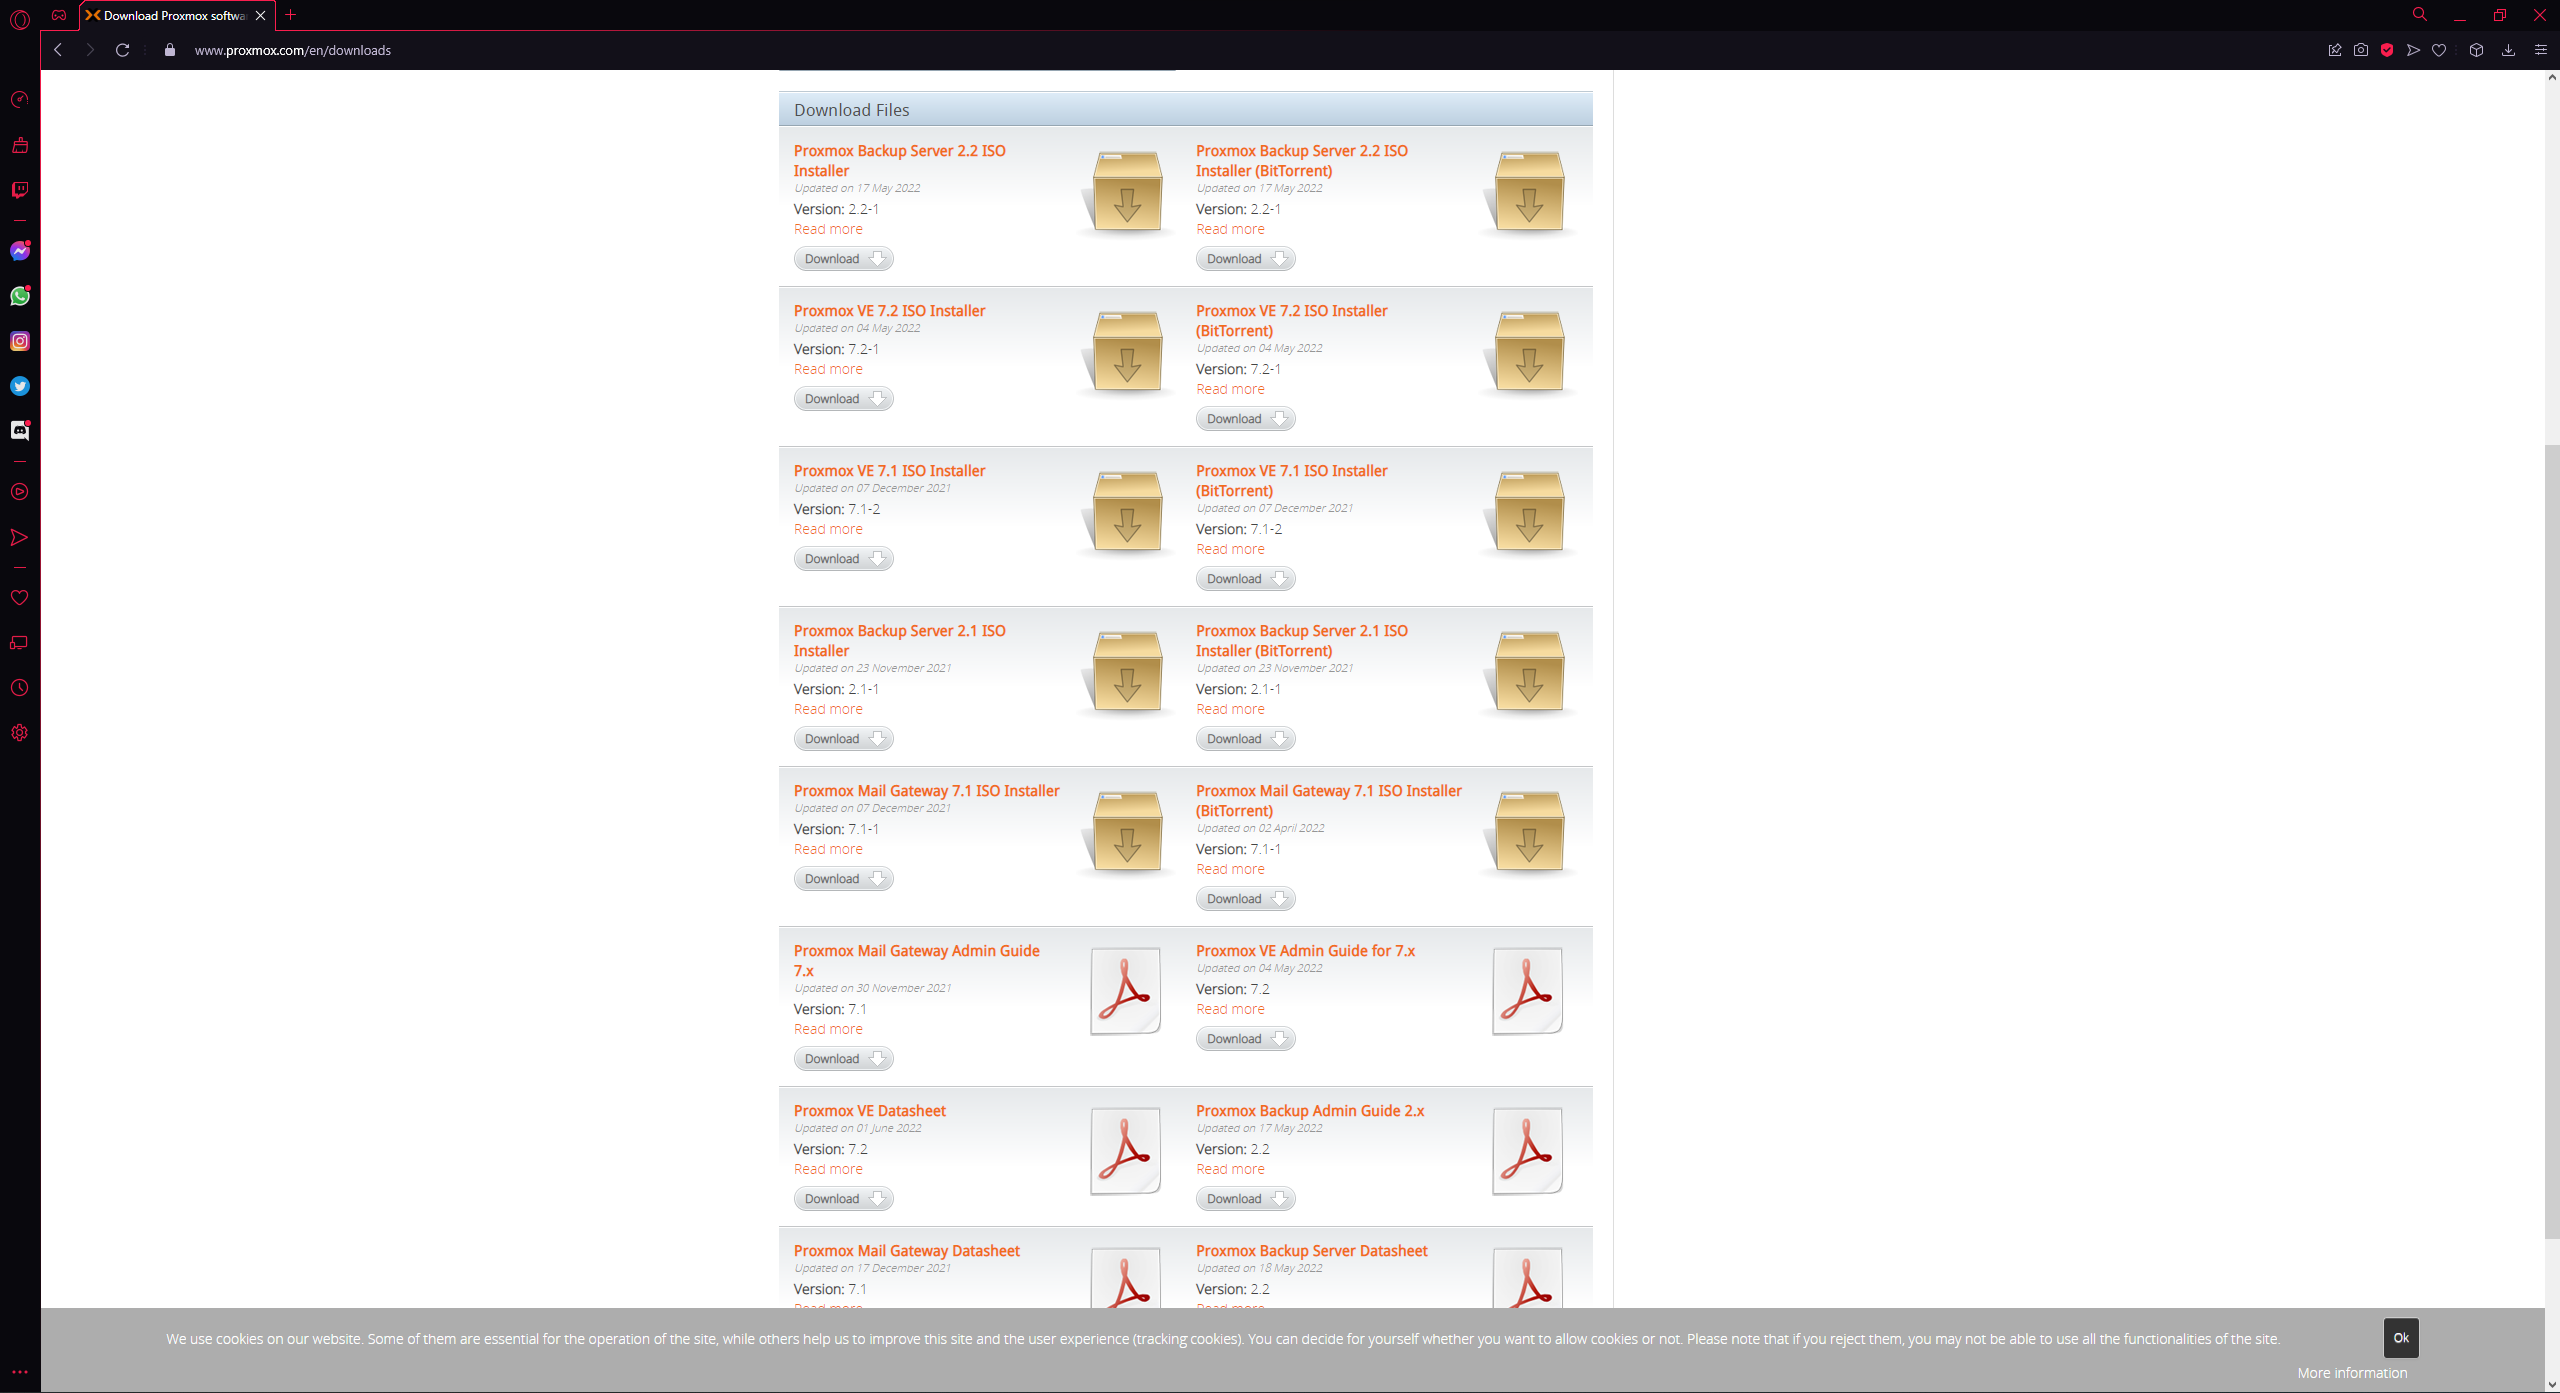
\includegraphics[width=1\linewidth]{proxmox web.png}
    \caption{web proxmox}
  \end{figure}
  \\ Setelah masuk ke website proxmox, tekan download pada salah satu list. Disarankan untuk mendownload Proxmox VE 7.1 ISO Installer
  \begin{figure}[h!]
    \centering
    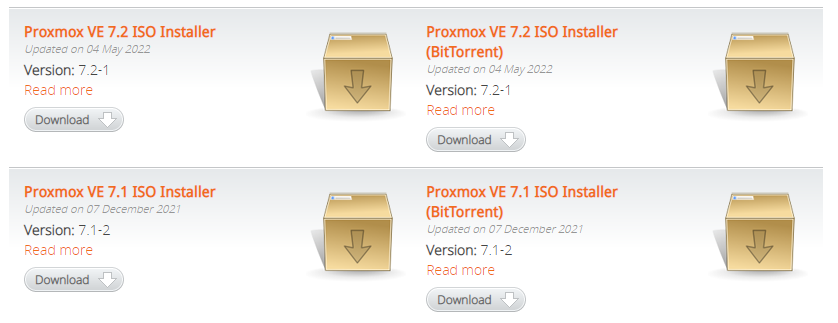
\includegraphics[width=1\linewidth]{proxmox download.png}
    \caption{download ISO}
  \end{figure}

  \newpage
  \subsection{Membuat Bootable}
  
\end{document}